\section{1-Lipschitz Neural Networks}\label{app:ortho}

We ensure that the kernel remains 1-Lipschitz by re-parametrizing them: $\Theta_i=\Pi(W_i)$ where $W_i$ is a set of unconstrained weights and $\Theta_i$ the orthogonal projection of $W_i$ on the Stiefel manifold - i.e the set of orthogonal matrices. The projection $\Pi$ is made with Bj\"orck algorithm~\cite{bjorck1971iterative}, which is differentiable and be included in the computation graph during forward pass. Unconstrained optimization is performed on $W_i$ directly.     

\section{Toy experiment in 2D}\label{app:toy2d}

All datasets are normalized to have zero mean and unit variance across all dimensions. The domain $B$ is chosen to be the ball of radius $5$. This guarantees that $\support\subset B$ for all datasets. The plots of figure\ref{fig:toy2d} are squares of sizes $[-5,5]$ for \textbf{(a)}, $[-3,3]$ for \textbf{(b)(c)(e)} and $[-4,4]$ for \textbf{(d)} to make the figure more appealing.     
  
\begin{figure}[!ht]
    \centering
    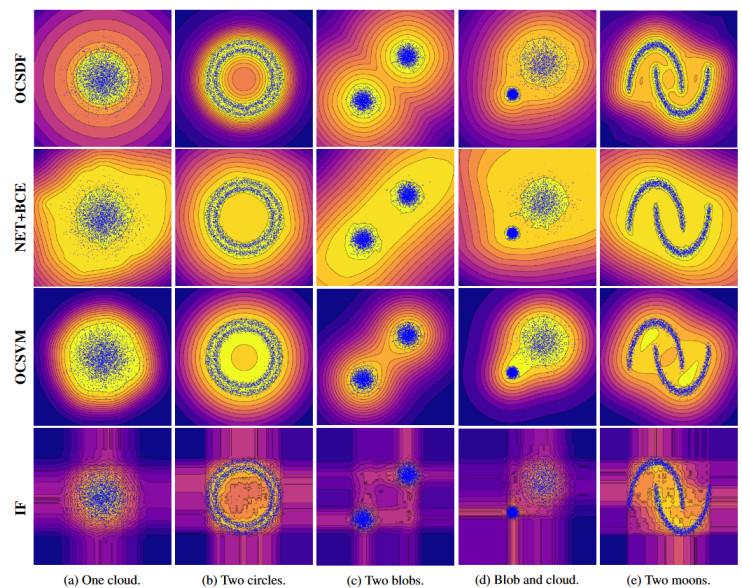
\includegraphics[width=\linewidth]{new_images/meshes/ocsdffinal.jpg}
    \caption{Toy examples of Scikit-learn. \textbf{Top row}: our method with Lipschitz (LIP) 1-Lipschitz network and $\hkr$ (HKR) loss. \textbf{Second row}: conventional network (NET) trained with Binary Cross Entropy (BCE). \textbf{Third row}: One Class SVM. \textbf{Fourth row}: Isolation Forest. }\label{fig:toy2dlarge}
    %Datasets: (a) One blob (b) Two circles (c) Two blobs (d) Two unbalanced blobs (e) Two moons.
\end{figure}

\iffalse
\begin{figure}[!ht]
    \centering
    
    \begin{subfigure}{0.02\textwidth}
    \rotatebox{90}{\textbf{OCSDF}} 
    \end{subfigure}
    \begin{subfigure}{0.19\textwidth}
        \centering
        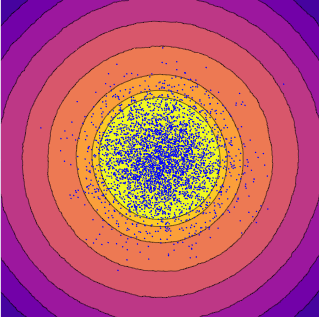
\includegraphics[width=1.\textwidth]{images/ocml/one-blob_cropped.png}
    \end{subfigure}
    \begin{subfigure}{.19\textwidth}
        \centering
        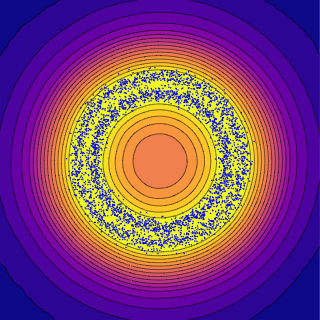
\includegraphics[width=1.\textwidth]{images/ocml/circles_cropped.png}
    \end{subfigure}
    \begin{subfigure}{0.19\textwidth}
        \centering
        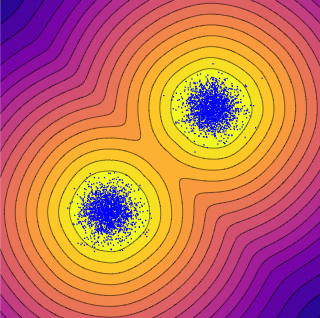
\includegraphics[width=1.\textwidth]{images/ocml/two_blobs_cropped.png}
    \end{subfigure}
    \begin{subfigure}{0.19\textwidth}
        \centering
        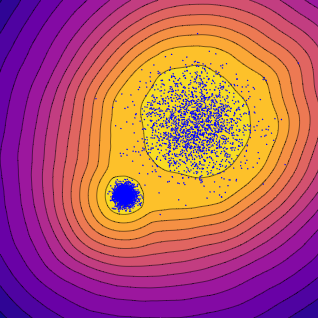
\includegraphics[width=1.\textwidth]{images/ocml/two-blobs-unbalanced_cropped.png}
    \end{subfigure}
    \begin{subfigure}{0.19\textwidth}
        \centering
        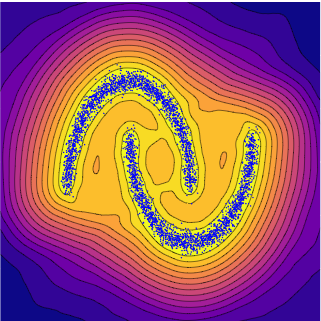
\includegraphics[width=1.\textwidth]{images/ocml/moons_cropped.png}
    \end{subfigure}
    
    %% OCSVM
    \begin{subfigure}{0.02\textwidth}
    \rotatebox{90}{\textbf{NET+BCE}} 
    \end{subfigure}
    \begin{subfigure}{0.19\textwidth}
        \centering
        
\includegraphics[width=1.\textwidth]{images/conventional/one-blob_cropped.png}
    \end{subfigure}
    \begin{subfigure}{.19\textwidth}
        \centering
        \includegraphics[width=1.\textwidth]{images/conventional/two-circles_cropped.png}
    \end{subfigure}
    \begin{subfigure}{0.19\textwidth}
        \centering
        \includegraphics[width=1.\textwidth]{images/conventional/two-blob_cropped.png}
    \end{subfigure}
    \begin{subfigure}{0.19\textwidth}
        \centering
        \includegraphics[width=1.\textwidth]{images/conventional/two-blob-unbalanced_cropped.png}
    \end{subfigure}
    \begin{subfigure}{0.19\textwidth}
        \centering
        \includegraphics[width=1.\textwidth]{images/conventional/two-moons_cropped.png}
    \end{subfigure}
    
    %% OCSVM
    \begin{subfigure}{0.02\textwidth}
    \rotatebox{90}{\textbf{OCSVM}} 
    \end{subfigure}
    \begin{subfigure}{0.19\textwidth}
        \centering
        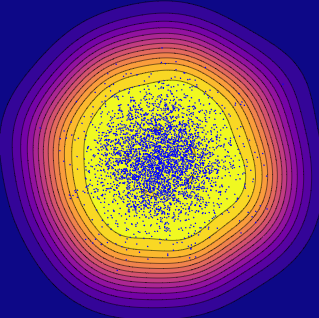
\includegraphics[width=1.\textwidth]{images/ocsvm/ocsvm_one-blob_cropped.png}
    \end{subfigure}
    \begin{subfigure}{.19\textwidth}
        \centering
        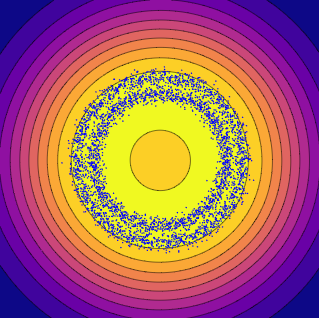
\includegraphics[width=1.\textwidth]{images/ocsvm/ocsvm_circles_cropped.png}
    \end{subfigure}
    \begin{subfigure}{0.19\textwidth}
        \centering
        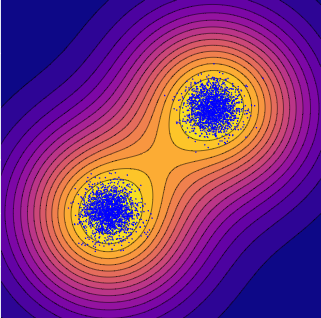
\includegraphics[width=1.\textwidth]{images/ocsvm/ocsvm_two_blobs_cropped.png}
    \end{subfigure}
    \begin{subfigure}{0.19\textwidth}
        \centering
        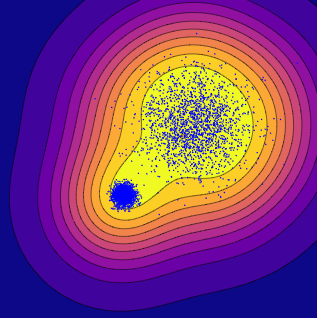
\includegraphics[width=1.\textwidth]{images/ocsvm/ocsvm_two-blobs-unbalanced_cropped.png}
    \end{subfigure}
    \begin{subfigure}{0.19\textwidth}
        \centering
        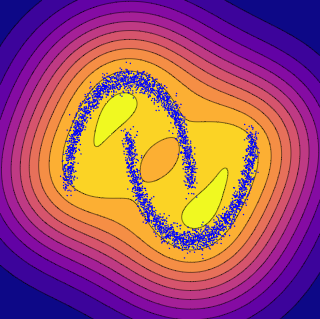
\includegraphics[width=1.\textwidth]{images/ocsvm/ocsvm_moons_cropped.png}
    \end{subfigure}
    
    %% IF
    \begin{subfigure}{0.02\textwidth}
    \rotatebox{90}{\textbf{IF}} 
    \end{subfigure}
    \begin{subfigure}{0.19\textwidth}
        \centering
        \includegraphics[width=1.\textwidth]{images/if/if_one-blob_cropped.png}
        \subcaption{One cloud.}
    \end{subfigure}
    \begin{subfigure}{.19\textwidth}
        \centering
        \includegraphics[width=1.\textwidth]{images/if/if_circles_cropped.png}
        \subcaption{Two circles.}
    \end{subfigure}
    \begin{subfigure}{0.19\textwidth}
        \centering
        \includegraphics[width=1.\textwidth]{images/if/if_two_blobs_cropped.png}
        \subcaption{Two blobs.}
    \end{subfigure}
    \begin{subfigure}{0.19\textwidth}
        \centering
        \includegraphics[width=1.\textwidth]{images/if/if_two-blobs-unbalanced_cropped.png}
        \subcaption{Blob and cloud.}
    \end{subfigure}
    \begin{subfigure}{0.19\textwidth}
        \centering
        \includegraphics[width=1.\textwidth]{images/if/if_moons_cropped.png}
        \subcaption{Two moons.}
    \end{subfigure}
    \caption{Toy examples of Scikit-learn. \textbf{Top row}: our method with Lipschitz (LIP) 1-Lipschitz network and $\hkr$ (HKR) loss. \textbf{Second row}: conventional network (NET) trained with Binary Cross Entropy (BCE). \textbf{Third row}: One Class SVM. \textbf{Fourth row}: Isolation Forest. }\label{fig:toy2dlarge}
    %Datasets: (a) One blob (b) Two circles (c) Two blobs (d) Two unbalanced blobs (e) Two moons.
\end{figure}
\fi

\subsection{One Class Learning}

All the toy experiments of figure~\ref{fig:toy2d} uses a $2\veryshortarrow512\veryshortarrow 512\veryshortarrow 512\veryshortarrow 512\veryshortarrow 1$ neural network. All the squares matrices are constrained to be orthogonal. The last layer is a unit norm column vector. The first layer consists of two unit norm columns that are orthogonal to each other. The optimizer is Rmsprop with default hyperparameters. The batch size is $b=256$, and the number of steps $T=4$ is small. We chose a margin $m=0.05$ except for ``blob and cloud'' dataset where we used $m=0.1$ instead. We take $\lambda=100$. The networks are trained for a total of $10,000$ gradient steps.    

\subsection{Other benchmarks}
  
For One Class SVM, we chose a parameter $\nu=0.05$, $\gamma=\frac{1}{2}$ (which corresponds to the ``scale'' behavior of scikit-learn for features in 2D with unit variance) and the popular RBF kernel. For Isolation Forest, we chose a default contamination level of $0.05$.   
  
The conventional network (without orthogonality constraint) is trained with Binary Cross Entropy (also called log-loss) and Adam optimizer. It shares the same architecture with ReLU instead of GroupSort. It is also trained for a total of $10,000$ gradient steps for a fair comparison. It would not make sense to use $\hkr$ loss for a conventional network since it diverges during training, as noticed in~\cite{bethune2022pay}. The Lipschitz constant of the conventional network grows uncontrollably during training even with Binary Cross-Entropy loss, which is also compliant with the results of~\cite{bethune2022pay}.  


\begin{figure}[!ht]
    \centering
    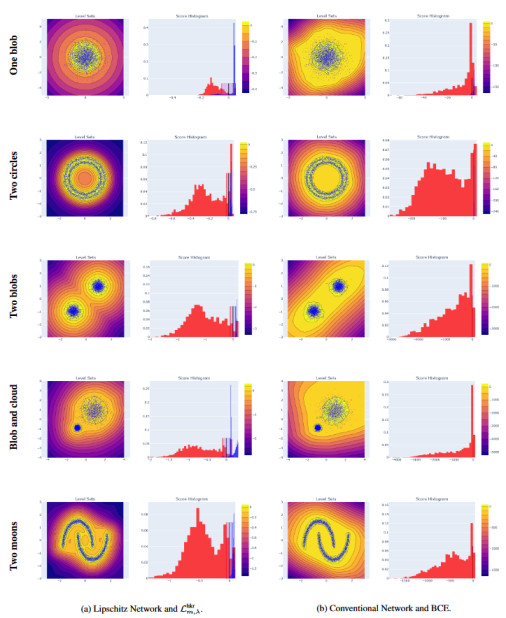
\includegraphics[width=\linewidth]{new_images/graphs/ocsdfhistogram.jpg}
    \caption{Histograms of score functions for 1-Lipschitz network (left) and conventional neural network. The blue bars correspond to the distribution of $f(x),x\sim\Prob_X$ and the red bars to the distribution $f(z),z\sim\Uniform(B)$.}\label{fig:toy2dhist}
\end{figure}


\iffalse
\begin{figure}[!ht]
    \centering
    
    \begin{subfigure}{0.02\textwidth}
    \rotatebox{90}{\textbf{One blob}} 
    \end{subfigure}
    \begin{subfigure}{0.48\textwidth}
        \centering
        \includegraphics[width=1.\textwidth]{images/ocml/one-blob.png}
    \end{subfigure}
    \begin{subfigure}{.48\textwidth}
        \centering
        \includegraphics[width=1.\textwidth]{images/conventional/one-blob.png}
    \end{subfigure}
    
    \begin{subfigure}{0.02\textwidth}
    \rotatebox{90}{\textbf{Two circles}} 
    \end{subfigure}
    \begin{subfigure}{0.48\textwidth}
        \centering
        \includegraphics[width=1.\textwidth]{images/ocml/circles.png}
    \end{subfigure}
    \begin{subfigure}{.48\textwidth}
        \centering
        \includegraphics[width=1.\textwidth]{images/conventional/two-circles.png}
    \end{subfigure}
    
    \begin{subfigure}{0.02\textwidth}
    \rotatebox{90}{\textbf{Two blobs}} 
    \end{subfigure}
    \begin{subfigure}{0.48\textwidth}
        \centering
        \includegraphics[width=1.\textwidth]{images/ocml/two_blobs.png}
    \end{subfigure}
    \begin{subfigure}{.48\textwidth}
        \centering
        \includegraphics[width=1.\textwidth]{images/conventional/two-blob.png}
    \end{subfigure}
    
    \begin{subfigure}{0.02\textwidth}
    \rotatebox{90}{\textbf{Blob and cloud}} 
    \end{subfigure}
    \begin{subfigure}{0.48\textwidth}
        \centering
        \includegraphics[width=1.\textwidth]{images/ocml/two-blobs-unbalanced.png}
    \end{subfigure}
    \begin{subfigure}{.48\textwidth}
        \centering
        \includegraphics[width=1.\textwidth]{images/conventional/two-blob-unbalanced.png}
    \end{subfigure}
    
    \begin{subfigure}{0.02\textwidth}
    \rotatebox{90}{\textbf{Two moons}} 
    \end{subfigure}
    \begin{subfigure}{0.48\textwidth}
        \centering
        \includegraphics[width=1.\textwidth]{images/ocml/moons.png}
        \subcaption{Lipschitz Network and $\hkr$.}
    \end{subfigure}
    \begin{subfigure}{.48\textwidth}
        \centering
        \includegraphics[width=1.\textwidth]{images/conventional/two-moons.png}
        \subcaption{Conventional Network and BCE.}
    \end{subfigure}
    
    \caption{Histograms of score functions for 1-Lipschitz network (left) and conventional neural network. The blue bars correspond to the distribution of $f(x),x\sim\Prob_X$ and the red bars to the distribution $f(z),z\sim\Uniform(B)$.}\label{fig:toy2dhist}
\end{figure}
\fi


\section{Toy experiments on 3D point clouds}\label{app:toy3d}

In figures~\ref{fig:cadtool1} and~\ref{fig:cadtool2}, we provide additional examples of the use of SDF to reconstruct shapes from point clouds. We also compare OCSDF with Deep SDF \cite{park2019deepsdf}, a standard baseline for neural implicit surface parametrization, to highlight the practical advantages of our method.

\begin{table}[ht]
    \centering
    %\hspace{-0.35cm}
    \small
    \begin{tabular}{c|cc}
    \hline
      \makecell{Methods\\} & \makecell{OCSDF\\ (ours)} & \makecell{DeepSDF\\ \cite{park2019deepsdf}}\\
    \hline
    %\hline
    Target & \makecell{Generate $Q\bedd P$} & \makecell{Compute $\Sdf(x)$ from $P$}\\
    Cost         & \makecell{Backward pass} & \makecell{Nearest Neighbor search} \\
    Loss         & HKR $\hkr$ & $\|f(x)-\Sdf(x)\|^2_2$\\
    Guarantees   & $f$ is 1-Lipschitz & None\\
    \end{tabular}
    \caption{Comparison of our approach against DeepSDF.}
    \label{tab:comparisondeepsdf}
\end{table}


\begin{figure}[!ht]
    \centering
    \includegraphics[width=1.\linewidth]{new_images/meshes/merged.png}
    \caption{SDF of $2048$ points sampled from the mesh of a 3D CAD model.}
    \label{fig:cadtool1}
\end{figure}

\begin{figure}[!ht]
    \centering
    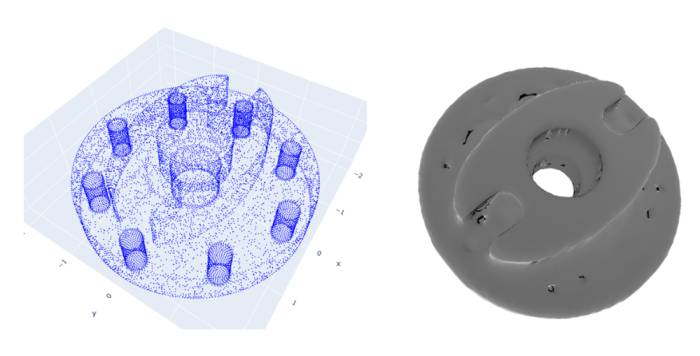
\includegraphics[width=0.7\linewidth]{new_images/meshes/hardtask.jpg}
    \caption{SDF of $2048$ points sampled from the mesh of a 3D CAD model.}
    \label{fig:cadtool2}
\end{figure}


\section{Tabular data}

The optimizer is RMSprop with default hyper-parameters. We use the lazy variant, i.e algorithm~\ref{alg:mmalgolazy}. We chose $\lambda=100$ and $m\in\{0.01, 0.05, 0.2, 1.\}$. The results are averaged over $20$ runs, and we report the highest average among all values of $m$. We use a batch size $b=128$ a number of steps $T=4$. The network is trained for a total of $40$ epochs over the one class, using a warm start of $5$ epoch with $T=0$.  

\paragraph{One Class (OC) protocol}: in this setting the normal examples are split in train and test set (approximately $50\%$ of data each). The network is trained on normal \textit{train} examples. The AUROC score is computed between  normal \textit{test} examples and anomalies. We report the results in table~\ref{tab:tabularrococ}.  

\paragraph{Anomaly Detection (AD) protocol}: in this setting the normal examples and anomalies are part of the train set. The network is trained on all examples. The AUROC score is computed between  normal examples and anomalies. We report the results in table~\ref{tab:tabularrocad}.  

\begin{table}%[]
    \centering
    \small
    %\hspace{-0.35cm}
    \begin{tabular}{ccc|c}
    \hline
      Dataset & $\bm{d}$ &\#train & OCSDF (Ours) \\
    \hline
    \hline
    Arrhythmia & 274 & 193 & $80.0\pm 1.3$\\
    Thyroid & 6 & 1,839 & $98.3\pm 0.1$\\     
    Mammography & 6 & 5,591 & $88.0\pm 1.4$\\
    Vowels & 12 & 703 & $96.1\pm 0.9$\\
    Satimage-2 & 36 & 2,866 & $97.8\pm 0.0$\\
    smtp & 3 & 47,553 & $83.8\pm 3.5$\\
    \end{tabular}
    \caption{AUROC score on \textit{test set + anomalies} with tabular data, averaged over $20$ runs. The dimension of the dataset is denoted by $\bm{d}$. In the \textbf{One Class protocol (OC)}, the classifier is trained on a subset of normal data, and test on unseen normal data and anomalous data. The ``\#train'' column indicates train set size.}
    \label{tab:tabularrococ}
\end{table}

\section{One Class Classification of image data}\label{app:occimage}

\subsection{Mnist experiment}

The MNIST images are normalized such that pixel intensity lies in $[-1,1]$ range. The set $B$ is chosen to be the image space, i.e $B=[-1,1]^{28\times 28}=[-1,1]^{784}$. The optimizer is RMSprop with default hyperparameters. We chose $m=0.02\times \sqrt{(28\times 28\times (1-(-1))}\approx 0.79$ : this corresponds to modification of $1$\% of the maximum norm of an image. We take $\lambda=200$. We use a batch size $b=128$, and a number of steps $T=16$. We use the lazy variant, i.e algorithm~\ref{alg:mmalgolazy}. The network is trained for a total of $70$ epochs over the one class (size of the support: $\approx 6000$ examples), using a warm start of $10$ epoch with $T=0$. The learning rate follows a linear decay from $1e^{-3}$ to $1e^{-6}$. 

All the experiments use a VGG-like architecture, depicted in table~\ref{tab:mnistarch}. Convolutions are parametrized using layers of Deel-Lip library~\cite{serrurier2021achieving}, which use an orthogonal kernel with a corrective constant on the upper bound of the Lipschitz constant of the kernel. Dense layers also use orthogonal kernels. We use \textit{l2-norm-pooling} layer with windows of size $2\times 2$ that operates as: $(x_{11},x_{12},x_{21},x_{22})\mapsto \|[x_{11},x_{12},x_{21},x_{22}]\|$.  
  
We see in table~\ref{tab:mnistroc} that it yields competitive results against other naive baselines such as Isolation Fortest (IF) or One Class SVM (OCSVM), and against the popular deep learning algorithm \textit{Deep SVDD}~\cite{ruff2018deep}.  

\paragraph{Against DeepSVDD.} We test 4 configurations for DeepSVDD.
\begin{enumerate}
    \item The one from the original's paper~\cite{ruff2018deep} with LeNet architecture.
    \item The Pytorch implementation from their official repository that combines LeNet and BatchNorm: \url{https://github.com/lukasruff/Deep-SVDD-PyTorch}.
    \item The Tensorflow implementation from pyod~\cite{zhao2019pyod} with dense layers and l$2$ activation regularization.
    \item The Tensorflow implementation from pyod but with the same (unconstrained) architecture as Table~\ref{tab:mnistarch} to ensure a fair comparison.
\end{enumerate}
Each configuration is run $10$ times, and the results are averaged. The best average among the four configurations is reported in the main paper, while we report in Table~\ref{tab:extensivedeepsvdd} the results of all the configurations. It appears that the method of the original paper is very sensitive to the network's architecture, and the results are hard to reproduce overall. Empirically, we also observe that the test/OOD AUROC is often smaller than train/OOD AUROC, which suggests that DeepSVDD memorizes the train set but do not generalize well outside of its train data. We also notice that those results are different from the ones originally reported by authors in their paper.   
  
\begin{table}%[]
    \centering
    \begin{tabular}{|c|cc|}
            \hline
            Datasets & Toy2D \& tabular\& Implicit Shape & Mnist \& Cifar-10 \\
            \hline
            \hline
            \# parameters & 792K  &  2,103K  \\
            \hline
            layer 1 &   dense-512 (fullsort)  &  conv-3x3-64 (groupsort)\\
            layer 2 &   dense-512 (fullsort)  &  conv-3x3-64 (groupsort)\\
            layer 3 &   dense-512 (fullsort)  &  conv-3x3-64 (groupsort)\\
            layer 4 &   dense-512 (fullsort)  &  conv-3x3-64 (groupsort)\\
            layer 5 &   dense-1 (linear)      &  l2 norm pooling - 2x2 \\
            layer 6 &                         &  conv-3x3-128 (groupsort)\\
            layer 7 &                         &  conv-3x3-128 (groupsort)\\
            layer 8 &                         &  conv-3x3-128 (groupsort)\\
            layer 9 &                         &  conv-3x3-128 (groupsort)\\
            layer 10 &                         &  l2 norm pooling - 2x2 \\
            layer 11 &                         &  conv-3x3-256 (groupsort)\\
            layer 12 &                         &  conv-3x3-256 (groupsort)\\
            layer 13 &                         &  conv-3x3-256 (groupsort)\\
            layer 14 &                         &  l2 norm pooling - 2x2 \\
            layer 15 &                         &  global l2 norm pooling \\
            layer 16 &                         &  dense-1 (linear) \\
            \hline
            \end{tabular}
    \caption{Architectures of the 1-Lipschitz networks used for the experiments, using layers of Deel-Lip library.}
    \label{tab:mnistarch}
\end{table}

\begin{table}%[]
    \centering
    \begin{tabular}{c|cccc}
            \hline
            Protocol & \makecell{As described\\ in article} & \makecell{As in Pytorch\\ repository} & \makecell{As in Pytorch repository\\ (best run)} & \makecell{Pyod\\ \cite{zhao2019pyod}}\\
            \hline
            \hline
            mean & $79.8\pm 2.9$ & $88.6\pm 6.1$ & $94.0\pm 3.6$ & $85.0\pm 7.8$\\
            \hline
            0 & $88.6\pm 0.$ & $90.2\pm 9.4$ & $97.2$ & $83.7\pm 0.$\\
            1 & $97.1\pm 0.$ & $99.6\pm 0.1$ & $99.7$ & $97.2\pm 0.$\\
            2 & $66.5\pm 0.$ & $79.9\pm 8.8$ & $88.8$ & $80.5\pm 0.$\\
            3 & $70.9\pm 0.$ & $80.5\pm 8.4$ & $91.3$ & $79.6\pm 0.$\\
            4 & $78.0\pm 0.$ & $88.3\pm 7.7$ & $93.9$ & $85.4\pm 0.$\\
            5 & $69.7\pm 0.$ & $82.8\pm 6.0$ & $89.5$ & $72.9\pm 0.$\\
            6 & $85.2\pm 0.$ & $95.8\pm 1.9$ & $97.8$ & $93.7\pm 0.$\\
            7 & $88.9\pm 0.$ & $91.0\pm 3.3$ & $94.7$ & $92.8\pm 0.$\\
            8 & $72.8\pm 0.$ & $84.6\pm 4.7$ & $90.5$ & $74.8\pm 0.$\\
            9 & $79.9\pm 0.$ & $93.3\pm 3.0$ & $96.1$ & $89.9\pm 0.$\\
            \end{tabular}
    \caption{Average AUROC over $10$ runs for each digit of Mnist. We re-code the method in \textit{Tensorflow} using various configurations, due to the discrepancies of protocols found in the literature. In overall, DeepSVDD is very sensitive to the network architecture and can dramatically overfit.}
    \label{tab:extensivedeepsvdd}
\end{table}
  
We report the histogram of predictions for the train set (One class), the set test (One class) and Out Of Distribution (OOD) examples (the classes of the test set) in figure~\ref{fig:mnisthisto}.  


\begin{figure}[!ht]
    \centering
    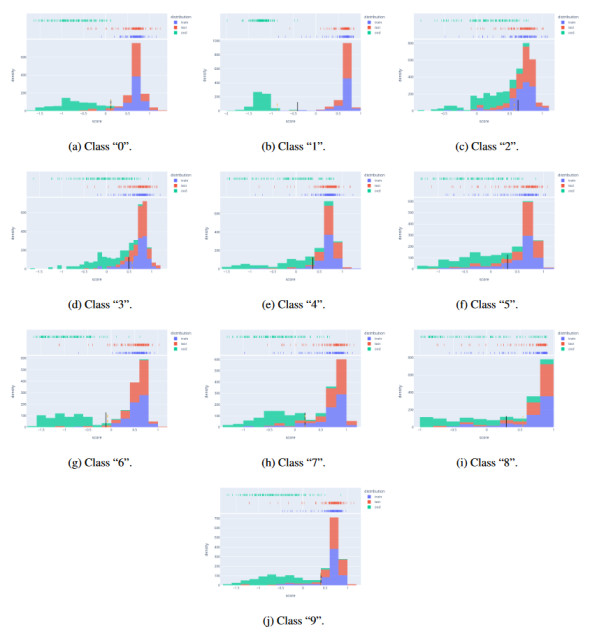
\includegraphics[width=\linewidth]{new_images/mnist/finalmnisthistograms.jpg}
    \caption{Histogram of scores predicted by the classifier at the end of training for \textbf{train} examples (in blue), \textbf{test} examples (in red), and \textbf{OOD Test} examples (in green) on Mnist after one of the runs of the algorithm.}\label{fig:mnisthisto}
\end{figure}


\iffalse
\begin{figure}[!ht]
    \centering
    
    %% 0 1 2
    \begin{subfigure}{0.3\textwidth}
        \centering
        \includegraphics[width=1.\textwidth]{images/mnist/histogram_0.png}
        \subcaption{Class ``0''.}
    \end{subfigure}
    \begin{subfigure}{.3\textwidth}
        \centering
        \includegraphics[width=1.\textwidth]{images/mnist/histogram_1.png}
        \subcaption{Class ``1''.}
    \end{subfigure}
    \begin{subfigure}{0.3\textwidth}
        \centering
        \includegraphics[width=1.\textwidth]{images/mnist/histogram_2.png}
        \subcaption{Class ``2''.}
    \end{subfigure}
    
    %% 3 4 5
    \begin{subfigure}{.3\textwidth}
        \centering
        \includegraphics[width=1.\textwidth]{images/mnist/histogram_3.png}
        \subcaption{Class ``3''.}
    \end{subfigure}
    \begin{subfigure}{0.3\textwidth}
        \centering
        \includegraphics[width=1.\textwidth]{images/mnist/histogram_4.png}
        \subcaption{Class ``4''.}
    \end{subfigure}
    \begin{subfigure}{.3\textwidth}
        \centering
        \includegraphics[width=1.\textwidth]{images/mnist/histogram_5.png}
        \subcaption{Class ``5''.}
    \end{subfigure}
    
    %% 6 7 8
    \begin{subfigure}{0.3\textwidth}
        \centering
        \includegraphics[width=1.\textwidth]{images/mnist/histogram_6.png}
        \subcaption{Class ``6''.}
    \end{subfigure}
    \begin{subfigure}{.3\textwidth}
        \centering
        \includegraphics[width=1.\textwidth]{images/mnist/histogram_7.png}
        \subcaption{Class ``7''.}
    \end{subfigure}
    \begin{subfigure}{0.3\textwidth}
        \centering
        \includegraphics[width=1.\textwidth]{images/mnist/histogram_8.png}
        \subcaption{Class ``8''.}
    \end{subfigure}
    
    %% 9
    \begin{subfigure}{.3\textwidth}
        \centering
        \includegraphics[width=1.\textwidth]{images/mnist/histogram_9.png}
        \subcaption{Class ``9''.}
    \end{subfigure}
    
    \caption{Histogram of scores predicted by the classifier at the end of training for \textbf{train} examples, \textbf{test} examples, and \textbf{OOD Test} examples on Mnist after one of the runs of the algorithm.}\label{fig:mnisthisto}
\end{figure}
\fi

\begin{table}%[]
    \centering
    \begin{tabular}{|c|ccccc|}
        \hline
       Dataset          & One cloud  & Two circles & Two blobs & Blob and cloud & Two moons \\
       \hline
       LLC conventional &   26.66    &    122.84   &  1421.41  &      53.90     &   258.73  \\ 
       \hline
    \end{tabular}
    \caption{Lower bound on the Local Lipschitz Constant (LLC) of the conventional network after $10,000$ training steps. It is obtained by computing the maximum of $\|\nabla_{x_i}f(x_i)\|$ over the train set. The LLC of the conventional network grows uncontrollably during training and fails to provide metric guarantees.}
    \label{tab:llc}
\end{table}

\subsection{Cifar-10}

The Cifar-10 images are centedered-reduced per channel (the certificates and the attacks take into account the rescaling in the computation of the radius). All pixel intensities fall in $[-2.1,2.14]$ interval. The set $B$ is chosen to be the image space, i.e $B=[-2.1,2.14]^{32\times 32\times 3}=[-2.1, 2.14]^{3072}$. The optimizer is RMSprop with default hyperparameters. We chose $m=0.002\times \sqrt{(32\times 32\times (2.14-(-2.1))}\approx 0.11$ : this corresponds to modification of $0.2$\% of the maximum norm of an image. We take $\lambda=1000$. We use a batch size $b=128$, and a number of steps $T=32$. We use the lazy variant, i.e algorithm~\ref{alg:mmalgolazy}. The network is trained for a total of $90$ epochs over the one class (size of the support: $\approx 5000$ examples), using a warm start of $10$ epoch with $T=0$. The learning rate follows a linear decay from $2.5e^{-4}$ to $2.5e^{-7}$.  

Note that the \textit{same} hyper-parameters are used for all the runs and all the classes. This is different from some practices of litterature (see fig~11. in~\cite{goyal_drocc_2020} ). Unfortunately this protocol is somewhat unfair since it explicitly leverages prior knowledge on the other classes - it can not be used in a real world scenario where the other classes are not available. Nonetheless, for completeness, we report in table~\ref{tab:cheatingprotocolcifar} the clean AUROC on Cifar10 with \textit{per class} tuning of the margin $m$.

\begin{table*}%[]
    \centering
    %\hspace{-0.35cm}
    \small
    \begin{tabular}{|cccccccccc|c|}
    \hline
    Airplane & Automobile & Bird & Cat & Deer & Dog & Frog & Horse & Ship & Truck & Mean\\
    \hline
    \hline
    $79.0$ & $65.2$ & $55.4$ & $60.4$ & $52.5$ & $56.9$ & $57.7$ & $55.0$ & $71.9$ & $67.0$ & $62.1\pm 8.0$\\
    \hline
    \end{tabular}
    \caption{Best AUROC of OCSDF on Cifar-10 with \textit{per class} tuning of the margin $m$.}
    \label{tab:cheatingprotocolcifar}
\end{table*}

\subsection{Empirical robustness}

We also report the complete results of the empirical robustness of OCSDF versus DeepSVDD for MNIST and Cifar10 in tables \ref{tab:empiricalmnistsvdd}, \ref{tab:empiricalOCSDFmnist}, \ref{tab:empiricalcifar10svdd} and \ref{tab:empiricalOCSDFcifar10}.

\begin{table*}%[]
    \centering
    %\hspace{-0.35cm}
    \small
    \begin{tabular}{|c|cccccc|}
    \hline
      Mnist & DeepSVDD & DeepSVDD & DeepSVDD & DeepSVDD & DeepSVDD & DeepSVDD \\
      l$2$-PGD & $\epsilon=8/255$ & $\epsilon=16/255$ & $\epsilon=36/255$ & $\epsilon=72/255$ & $\epsilon=144/255$ & $\epsilon=255/255$\\
    \hline
    \hline
    mean & $90.2\pm 6.4$ & $89.7\pm 6.9$ & $88.2\pm 8.4$ & $84.5\pm 12.2$ & $74.1\pm 21.7$ & $61.9\pm 29.0$\\
    \hline
    digit 0 & $96.9$ & $96.5$ & $95.3$ & $91.6$ & $78.8$ & $56.9$\\
    digit 1 & $99.6$ & $99.6$ & $99.6$ & $99.5$ & $99.5$ & $99.4$\\
    digit 2 & $80.6$ & $78.9$ & $73.7$ & $61.2$ & $29.4$ & $08.4$\\
    digit 3 & $87.2$ & $86.7$ & $85.4$ & $82.2$ & $69.6$ & $47.8$\\
    digit 4 & $90.7$ & $90.7$ & $90.7$ & $90.5$ & $90.0$ & $89.4$\\
    digit 5 & $83.0$ & $81.5$ & $76.7$ & $65.9$ & $44.2$ & $28.8$\\
    digit 6 & $97.7$ & $97.6$ & $97.0$ & $95.2$ & $86.8$ & $69.2$\\
    digit 7 & $93.3$ & $93.2$ & $92.9$ & $92.4$ & $90.9$ & $89.4$\\
    digit 8 & $82.7$ & $82.1$ & $80.3$ & $76.1$ & $61.5$ & $39.7$\\
    digit 9 & $90.5$ & $90.5$ & $90.4$ & $90.4$ & $90.2$ & $89.7$\\
    \hline
    \end{tabular}
    \caption{Empirical AUROC against l$2$-PGD adversarial attacks on Mnist for DeepSVDD.}
    \label{tab:empiricalmnistsvdd}
\end{table*}

\begin{table*}%[]
    \centering
    %\hspace{-0.35cm}
    \small
    \begin{tabular}{|c|cccccc|}
    \hline
      Mnist & OCSDF & OCSDF & OCSDF & OCSDF & OCSDF & OCSDF \\
      l$2$-PGD & $\epsilon=8/255$ & $\epsilon=16/255$ & $\epsilon=36/255$ & $\epsilon=72/255$ & $\epsilon=144/255$ & $\epsilon=255/255$\\
    \hline
    \hline
    mean & $93.2\pm 5.0$ & $92.8\pm 5.3$ & $91.8\pm 6.0$ & $89.8\pm 7.4$ & $83.1\pm 11.9$ & $68.2\pm 19.5$\\
    \hline
    digit 0 & $99.4$ & $99.4$ & $99.3$ & $99.1$ & $98.2$ & $94.9$\\
    digit 1 & $99.1$ & $99.0$ & $98.8$ & $98.4$ & $96.7$ & $90.9$\\
    digit 2 & $89.7$ & $89.1$ & $87.5$ & $84.4$ & $74.0$ & $51.0$\\
    digit 3 & $91.1$ & $90.5$ & $89.2$ & $86.4$ & $77.3$ & $56.6$\\
    digit 4 & $95.2$ & $94.9$ & $94.1$ & $92.6$ & $87.1$ & $73.0$\\
    digit 5 & $84.6$ & $83.7$ & $81.2$ & $76.3$ & $60.8$ & $33.3$\\
    digit 6 & $98.0$ & $97.9$ & $97.6$ & $96.9$ & $94.4$ & $86.9$\\
    digit 7 & $95.3$ & $95.0$ & $94.4$ & $93.0$ & $88.5$ & $77.2$\\
    digit 8 & $85.8$ & $85.1$ & $83.3$ & $79.7$ & $68.7$ & $46.9$\\
    digit 9 & $93.9$ & $93.6$ & $92.7$ & $91.0$ & $85.2$ & $70.9$\\
    \hline
    \end{tabular}
    \caption{Empirical AUROC against l$2$-PGD adversarial attacks on Mnist for one run of OCSDF in One Class learning.}
    \label{tab:empiricalOCSDFmnist}
\end{table*}

\begin{table*}%[]
    \centering
    %\hspace{-0.35cm}
    \small
    \begin{tabular}{|c|cccccc|}
    \hline
      CIFAR10 & DeepSVDD & DeepSVDD & DeepSVDD & DeepSVDD & DeepSVDD & DeepSVDD \\
      l$2$-PGD & $\epsilon=8/255$ & $\epsilon=16/255$ & $\epsilon=36/255$ & $\epsilon=72/255$ & $\epsilon=144/255$ & $\epsilon=255/255$\\
    \hline
    \hline
    mean & $54.4\pm 8.3$ & $46.5\pm 8.1$ & $28.4\pm 7.0$ & $09.2\pm 3.7$ & $0.7\pm 0.6$ & $0.1\pm 0.0$\\
    \hline
    Airplane & $62.82$ & $55.09$ & $36.21$ & $12.57$ & $0.76$ & $0.01$\\
    Automobile & $43.02$ & $36.94$ & $21.98$ & $8.35$ & $1.24$ & $0.09$\\
    Bird & $58.50$ & $49.13$ & $27.66$ & $6.47$ & $0.16$ & $0.01$\\
    Cat & $45.80$ & $36.82$ & $18.76$ & $3.91$ & $0.12$ & $0.00$\\
    Deer & $63.02$ & $53.55$ & $30.82$ & $7.41$ & $0.23$ & $0.00$\\
    Dog & $50.33$ & $43.32$ & $27.95$ & $10.88$ & $1.43$ & $0.09$\\
    Frog & $63.44$ & $55.31$ & $35.33$ & $11.12$ & $0.63$ & $0.01$\\
    Horse & $44.67$ & $36.55$ & $20.09$ & $5.37$ & $0.26$ & $0.00$\\
    Ship & $64.38$ & $57.67$ & $40.89$ & $17.47$ & $1.87$ & $0.04$\\
    Truck & $48.39$ & $40.85$ & $24.79$ & $8.46$ & $0.81$ & $0.03$\\
    \hline
    \end{tabular}
    \caption{Empirical AUROC against l$2$-PGD adversarial attacks on Cifar10 for DeepSVDD.}
    \label{tab:empiricalcifar10svdd}
\end{table*}

\begin{table*}%[]
    \centering
    %\hspace{-0.35cm}
    \small
    \begin{tabular}{|c|cccccc|}
    \hline
      CIFAR10 & OCSDF & OCSDF & OCSDF & OCSDF & OCSDF & OCSDF \\
      l$2$-PGD & $\epsilon=8/255$ & $\epsilon=16/255$ & $\epsilon=36/255$ & $\epsilon=72/255$ & $\epsilon=144/255$ & $\epsilon=255/255$\\
    \hline
    \hline
    mean & $59.0\pm 9.3$ & $58.2\pm 9.2$ & $56.7\pm 9.6$ & $53.9\pm 10.3$ & $48.4\pm 10.3$ & $39.8\pm 13.8$\\
    \hline
    Airplane & $80.1$ & $79.8$ & $79.0$ & $77.4$ & $73.9$ & $67.6$\\
    Automobile & $60.2$ & $59.5$ & $57.7$ & $54.4$ & $47.3$ & $35.7$\\
    Bird & $52.7$ & $51.9$ & $49.9$ & $46.2$ & $38.8$ & $28.0$\\
    Cat & $57.7$ & $57.0$ & $55.4$ & $52.3$ & $46.1$ & $36.6$\\
    Deer & $50.8$ & $50.0$ & $48.0$ & $44.4$ & $37.3$ & $27.1$\\
    Dog & $55.8$ & $55.2$ & $53.5$ & $50.5$ & $44.4$ & $35.0$\\
    Frog & $54.7$ & $54.0$ & $52.2$ & $49.1$ & $42.8$ & $32.9$\\
    Horse & $48.0$ & $47.3$ & $45.4$ & $42.0$ & $35.3$ & $25.5$\\
    Ship & $71.7$ & $69.2$ & $68.7$ & $67.5$ & $65.1$ & $61.5$\\
    Truck & $57.9$ & $57.6$ & $56.9$ & $55.4$ & $52.5$ & $48.1$\\
    \hline
    \end{tabular}
    \caption{Empirical AUROC against l$2$-PGD adversarial attacks on Cifar10 for one run of OCSDF in One Class learning.}
    \label{tab:empiricalOCSDFcifar10}
\end{table*}

\subsection{Image synthesis from One Class classifier}

We perform a total of $T=64$ steps with algorithm~\ref{alg:newtonraphson} by targeting the level set $f^{-1}(\{\Expect_{\Prob_X}[f(x)]\})$ (to ensure we stay inside the distribution). Moreover, during image synthesis, we follow a deterministic path by setting $\eta=1$. The images generated were picked randomly (with respect to initial sample $z_0\sim\Uniform(B)$) without cherry-picking. Interestingly, we see that the algorithm recovers some \textit{in-distribution} examples successfully.    
The examples for which the image is visually deceptive are somewhat correlated with low AUC scores. Those failure cases are also shared by concurrent methods, which suggests that some classes are harder to distinguish. Notice that sometimes Out Of Distribution (OOD) Mnist digits, from \textit{other classes not seen during training}, are sometimes generated. This suggests that most Mnist digits can be built from a small set of elementary features that are combined during the generation of $Q_t$. Visualizations of generated digits are presented in Figure \ref{fig:mnist_gen}.

\begin{figure}[!ht]
    \centering
    
    %% 0 1
    \begin{subfigure}{0.4\textwidth}
        \centering
        
\includegraphics[width=1.\textwidth]{new_images/mnist/gan_0_cropped.PNG}
    \end{subfigure}\begin{subfigure}{0.4\textwidth}
        \centering
        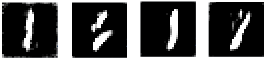
\includegraphics[width=1.\textwidth]{new_images/mnist/gan_1_cropped.png}
    \end{subfigure}
    
    %% 2 3
    \begin{subfigure}{0.4\textwidth}
        \centering
        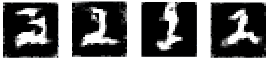
\includegraphics[width=1.\textwidth]{new_images/mnist/gan_2_cropped.png}
    \end{subfigure}\begin{subfigure}{0.4\textwidth}
        \centering
        
\includegraphics[width=1.\textwidth]{new_images/mnist/gan_3_cropped.png}
    \end{subfigure}
    
    %% 4 5
    \begin{subfigure}{0.4\textwidth}
        \centering
        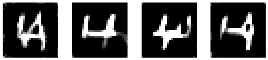
\includegraphics[width=1.\textwidth]{new_images/mnist/gan_4_cropped.png}
    \end{subfigure}\begin{subfigure}{0.4\textwidth}
        \centering
        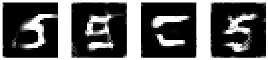
\includegraphics[width=1.\textwidth]{new_images/mnist/gan_5_cropped.png}
    \end{subfigure}
    
    %% 6 7
    \begin{subfigure}{0.4\textwidth}
        \centering
        
\includegraphics[width=1.\textwidth]{new_images/mnist/gan_6_cropped.png}
    \end{subfigure}\begin{subfigure}{0.4\textwidth}
        \centering
        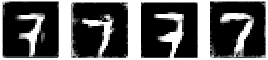
\includegraphics[width=1.\textwidth]{new_images/mnist/gan_7_cropped.png}
    \end{subfigure}
    
    
    %% 8 9
    \begin{subfigure}{0.4\textwidth}
        \centering
        
\includegraphics[width=1.\textwidth]{new_images/mnist/gan_8_cropped.png}
    \end{subfigure}\begin{subfigure}{0.4\textwidth}
        \centering
        
\includegraphics[width=1.\textwidth]{new_images/mnist/gan_9_cropped.png}
    \end{subfigure}
    
    \caption{Synthetic examples obtained by running algorithm~\ref{alg:newtonraphson} with $T=64$ and $\eta=1$.}\label{fig:mnist_gen}
    %Datasets: (a) One blob (b) Two circles (c) Two blobs (d) Two unbalanced blobs (e) Two moons.
\end{figure}
  
Finally, note that our method is not tailored for example generation: this is merely a side effect of the training process of the classifier. There is no need a the encoder-decoder pair of VAE nor the discriminator-generator pair of a GAN. Moreover, no hyper-parameters other than $m$ and $T$ are required.   

\section{Known Limitations}\label{app:limitations}

Despite its performance and appealing properties, the method suffers from some important limitations we highlight below and that can serve as a basis for future work. 

\subsection{Gradient Norm Preserving networks (GNP) approximation power}

The performance of the algorithm strongly depends on its capacity to properly learn the true minimizer $f^{*}$ of $\hkr$ loss. Per Property~\ref{prop:gnphkr} such minimizer must fulfill $\|\nabla_x f^{*}(x)\|_2=1$ everywhere on the support of $\Prob_X$ and $Q_t$. Hence the performance of the algorithm (and the associated theoretical guarantees) depends on the capacity of the GNP network to fulfil this property. In the tabular case, it is easy to do using orthogonal matrices for affine layers and GroupSort (or FullSort~\cite{anil2019sorting}) activation functions. However, in the image case, designing ``orthogonal convolution'' is still an active research area. Several solutions have been proposed, but they come with various drawbacks in terms of simplicity of implementation, computational cost, or tightness of the constraint. Hence the average gradient norm on image datasets struggles to exceed $0.3$ in practice. Another limitation stems from low-rank adjoint operators (e.g the last layer of the network): during backpropagation they do not preserve gradient norm along all directions.  
  
The Newton-Raphson trick that uses steps of size $\frac{\nabla_x f(x)}{\|\nabla_x f(x)\|_2^2}$ mitigates partially the issue. This suggests that the algorithm (in its current form) could benefit from further progress in Gradient Norm Preserving (GNP) architectures.  

\subsection{Limitations of the euclidean norm in image space}

The algorithm provides metric guarantees in the construction of the Signed Distance Function (SDF) to the boundary. The $l2$-norm is not a crucial component of the construction: the proof of~\ref{thm:hkrsdf} and Proposition 2 of~\cite{serrurier2021achieving} can be applied to any norm. However, in every case, the Lipschitz constraint $|f(x)-f(y)|\leq \|x-y\|_L$ on the network architecture must coincide with the norm $\|\cdot\|_L$ used to build the signed distance function. Currently, only networks that are Lipschitz with respect to $l^{\infty}$ and $l^2$ norms benefit from universal approximation properties~\cite{anil2019sorting}. Those norms are often meaningful for tabular data, but not for images. Hence, metric guarantees are less useful in pixel space. The method still benefits from certificates against adversarial attacks, which is highly desirable for critical systems but lacks semantic interpretation otherwise.  

\subsection{Tuning of margin}

The algorithm is not quite agnostic to the data: the margin $m>0$ used in $\hkr$ loss is an important parameter that serves as prior on the typical distance that separates the One Class support from the anomalies. This hyper-parameter can be guessed from the final application at hand (very much like the ``scale'' parameter of radial basis function kernels), manually with grid search algorithms or more extensive procedures. Theorem~\ref{thm:hkrsdf} suggests that a small margin $m$ works best. However, the VC dimension associated with the corresponding set of classifiers increases polynomially with $\frac{1}{m}$ (see Proposition 6 of~\cite{bethune2022pay}). Hence, the algorithm benefits from faster convergence and more stability during training when $m$ is big. Fortunately, this tradeoff present in most deep learning-based algorithms is solely controlled by this one-dimensional parameter in our case. Any heuristic estimation from data or with a one-dimensional line search is feasible, even with a limited computational budget.  

\section{Hardware}\label{app:hardware}

The hardware consists of a workstation with NVIDIA 1080 GPU with 8GB memory and a machine with 32GB RAM. Hence, while being based on deep learning, and obviously benefiting from faster hardware, the requirements are affordable to most practitioners. The typical duration of an epoch on most challenging datasets was under a minute.    
